\documentclass[11pt]{beamer} 
\usepackage[spanish]{babel}
\usepackage[utf8]{inputenc}

\usepackage{lmodern}
\usepackage[T1]{fontenc}
\usepackage{textcomp}

\usetheme{Copenhagen}
\usecolortheme{seagull}

\usepackage{tikz}
\usetikzlibrary{mindmap,trees}
\usepackage{tikz-er2}

\title{\bf Babel}
\author{Carlos Caballero}
\institute{scesi}

\begin{document}

\begin{frame}
\hspace*{3.5cm}

\includegraphics[width=0.32\textwidth]{img/babel.png}
\titlepage
\end{frame}

\section{Definición}
\begin{frame}
Babel es la primera pieza de un proyecto destinado a minimizar las dificultades
que generalmente se sufren en el contexto en el que nos desempeñamos.
\end{frame}

\subsection{Los problemas}
\begin{frame}
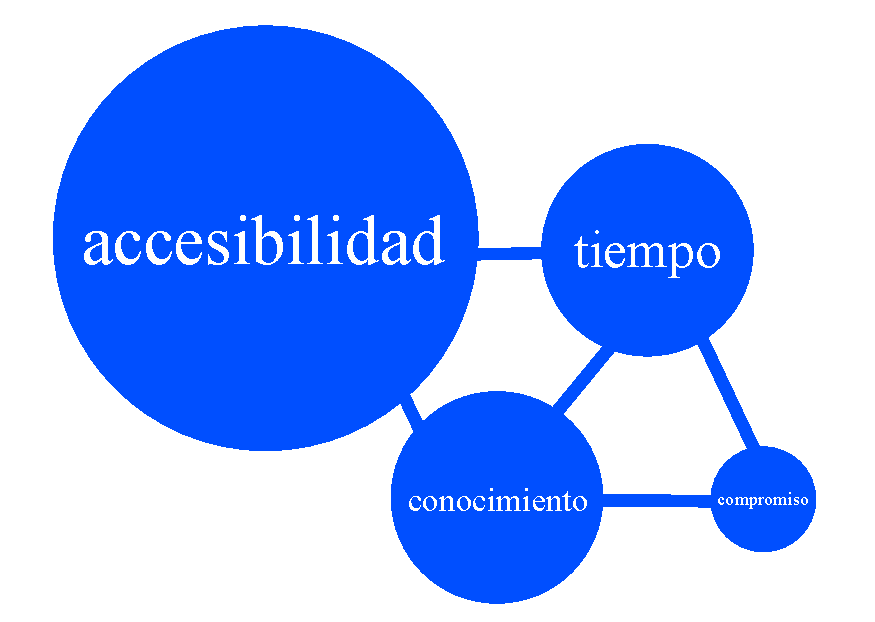
\includegraphics[width=1.0\textwidth]{img/babel_1.pdf}
\end{frame}

\subsection{Funciones}
\begin{frame}
Babel es un sistema web que ofrece acceso a una colección de documentos en formato pdf.\\ \pause
Posee las siguientes caracteristicas: \pause
\begin{itemize}
\item Los documentos son compartidos por sus usuarios. \pause
\item Estos son revisados, clasificados y publicados por sus administradores. \pause
\item Cualquier persona puede descargar, catalogar y valorar los documentos de manera anonima.
\end{itemize}
\end{frame}

\subsection{Premisas}
\begin{frame}
Este sistema se construyó siguiendo las premisas citadas a continuación:\\ \pause
\begin{itemize}
\item Maximizar el anonimato de todos sus usuarios. \pause
\item Dinamizar el conjunto de posibilidades de clasificación. \pause
\item Ofrecer amplias formas de automatización de tareas comunes.
\end{itemize}
\end{frame}

\end{document}
